% !TEX program = xelatex
\documentclass[notes=show]{beamer}
%\documentclass[notes=hide]{beamer}
%\documentclass[notes=only]{beamer}
%\documentclass[handout]{beamer}

\usepackage{newtxtext}
\usepackage{analchem}
\usepackage{lecture}

\graphicspath{{./Figures/},{./spec/}}

\title{Spectrophotometry}
\institute{CHEM321 --- Analytical Chemistry I \\ Bloomsburg University}
\author{D.A. McCurry}
\date{Fall 2021}

\begin{document}

%% PART 1

\maketitle
\mode<article>{\thispagestyle{fancy}}

\frame{\section{Fundamentals}
	\begin{learningobjectives}
	\item Relate wavelength of light to energy.
	\item Identify regions of electromagnetic radiation suitable for
		particular analyses.
	\item Qualitatively describe how light can be absorbed by molecules.
	\end{learningobjectives}
}

\begin{frame}{Spectrophotometry}
	Any procedure that uses light (electromagnetic radiation) to measure
	chemical concentrations.

	\bigskip

	\begin{block}{Electromagnetic Radiation (EMR)}
		\begin{itemize}
			\item Energy radiated in the form of a \alert{wave}
				caused by an electric field interacting with a
				magnetic field.
			\item Result of the acceleration of a charged particle.
			\item Does not require a material medium and can travel
				through a vacuum.
		\end{itemize}
	\end{block}
\end{frame}


\begin{frame}{Properties of EMR}
	\note{%
	\begin{center}
		\begin{tabularx}{0.8\linewidth} {>{$}r<{$}@{ = }X}
			\multicolumn{2}{c}{$c = \nu \lambda_i$} \\[1em]
			c & speed of light in vacuum,
			\SI{2.998e8}{\meter\per\second} \\
			\nu & frequency \\
			\lambda_i & wavelength \\[1.5em]
			\multicolumn{2}{c}{$E = h\nu$} \\[1em]
			E & energy of radiation \\
			h & Planck's constant, \SI{6.626e-34}{\joule\second}
			\\[2em]
		\end{tabularx}
		\fbox{Combining yields: $E = \dfrac{hc}{\lambda_i}$}
	\end{center}
}

	\begin{center}
		\includegraphics[width=\linewidth]{EMRproperties.png}
	\end{center}
\end{frame}

\begin{frame}{Regions of the Electromagnetic Spectrum}
	\includegraphics[width=\linewidth]{EM_Spectrum_Properties_edit.pdf}

	\footnotesize{By Inductiveload, NASA [GFDL
	(http://www.gnu.org/copyleft/fdl.html) or CC-BY-SA-3.0
	(http://creativecommons.org/licenses/by-sa/3.0/)], via Wikimedia
	Commons}
\end{frame}

\begin{frame}[allowframebreaks]{Molecular Processes}
	The net energy ($E$) of a molecule consists of all energies applied to
	it: \alert{translational}, \alert{rotational}, \alert{vibrational}, and
	\alert{electronic energy} (major terms).
	\begin{multline*}
		E_\text{molecule} = E_\text{nuclear spin} + E_\text{electron
		spin} + E_\text{translational} \\ + E_\text{rotation} +
		E_\text{vibration} + E_\text{electronic}
	\end{multline*}

	\begin{description}
		\item[Spin       ] nuclear and electron spin
		\item[Translation] movement of the molecule through space
		\item[Rotation   ] rotation of the molecule
		\item[Vibration  ] vibration of the atoms with respect to each other
		\item[Electronic ] mutual interactions of the electrons and nuclei
\end{description}

\framebreak

	\begin{tikzpicture}
		\node(molproc)
			{\includegraphics[width=\linewidth,trim={0 120pt 0
			0},clip]{EMRmolecules.png}};
		\node[below = 0pt of molproc,text width=\linewidth,align=center]
			{All these energy states \alert{except} translational
				(stationary states) are
		\alert{quantized}.};
	\end{tikzpicture}
\end{frame}

\begin{frame}[allowframebreaks]{Absorption of Light}
	\begin{columns}
		\column{0.5\linewidth}
		\begin{center}
			\scalebox{0.75}{
				\documentclass{standalone}

\usepackage{tikz}

\begin{document}

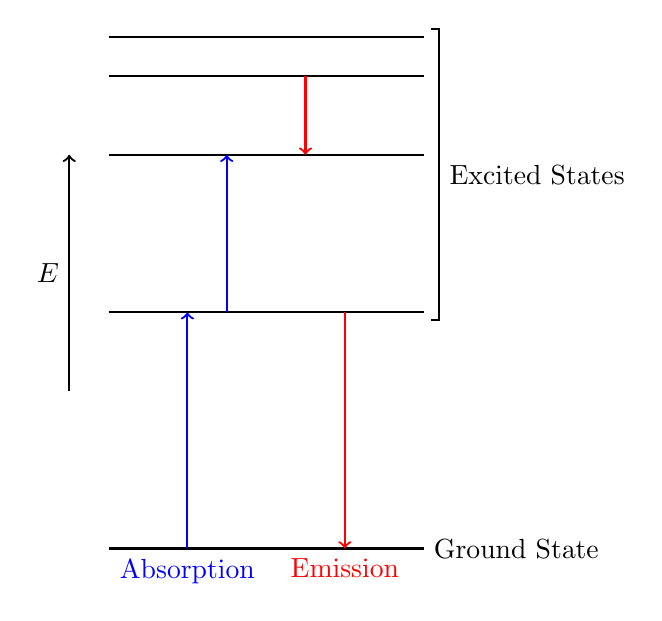
\begin{tikzpicture}[every path/.style={thick}]
	\draw (0,0) -- (4,0) node[right] {Ground State};
	\draw (0,3) -- (4,3);
	\draw (0,5) -- (4,5);
	\draw (0,6) -- (4,6);
	\draw (0,6.5) -- (4,6.5);
	\draw[->,blue] (1,0) -- (1,3) node[pos=0,below] {Absorption};
	\draw[->,blue] (1.5,3) -- (1.5,5);
	\draw[->,red] (2.5,6) -- (2.5,5);
	\draw[->,red] (3,3) -- (3,0) node[pos=1,below] {Emission};
	\draw (4.1,6.6) -- (4.2,6.6) -- (4.2,2.9) node[midway,right] {Excited
	States} -- (4.1,2.9);
	\draw[->] (-0.5,2) -- (-0.5,5) node[midway,left] {$E$};
\end{tikzpicture}

\end{document}
}
		\end{center}
		\column{0.4\linewidth}
		\begin{itemize}
			\item When EMR is \alert{absorbed}, the molecule is
				\alert{excited} to a higher \alert{energy
				state}.
			\item Relaxation, or \alert{emission}, is associated
				with the release of a photon (or heat).
		\end{itemize}
	\end{columns}

	\framebreak

	Consider formaldehyde, \ch{CH2O}:
	\begin{center}
		\includegraphics[width=0.6\linewidth]{formaldehyde.png}
	\end{center}
	The \alert{excited state}, $S_1$, has a slightly different geometry due
	to an \alert{electronic transition} of an electron from one
	\alert{molecular orbital} to another.
	\begin{center}
		\begin{tabular} {>{$}c<{$} c l}
			S_i & \alert{singlet} state & electron spins opposed \\
			T_i & \alert{triplet} state & electron spins parallel
		\end{tabular}
	\end{center}

	\framebreak

	\begin{columns}
		\column{0.5\textwidth}
		\includegraphics[width=\linewidth]{formaldehyde-mo.png}
		\column{0.5\textwidth}
		\begin{itemize}
			\item Absorption of UV and visible light promotes
				electronic transitions in formaldehyde.
			\item Microwave or infrared radiation do not contain
				enough energy to induce such transitions.
				\begin{itemize}
					\item They \alert{can} change the
						vibrational or rotational motion
						of the molecule, however!
				\end{itemize}
		\end{itemize}
	\end{columns}

	\framebreak

	\begin{center}
		\includegraphics[width=0.8\linewidth]{formaldehyde-vibration.png}
	\end{center}

	Vibrational transitions usually involve simultaneous rotational
	transitions. Electronic transitions usually involve simultaneous
	vibrational and rotational transitions.

	\framebreak

	We can measure the amount of incident EMR absorbed using a
	spectrophotometer:
	\begin{center}
		\includegraphics[width=0.8\linewidth]{spectrometer.png}
	\end{center}

	\begin{tabularx}{\linewidth} {>{$}r<{$}@{ = }X}
		P_0 & Incident \alert{irradiance} (energy per second per unit
		area, \si{\watt\per\meter\squared}) \\
		P & Irradiance leaving sample \\
		b & length of path through sample
	\end{tabularx}

	\begin{center}
		\fbox{We can measure the relationship between $P_0$ and $P$!}
	\end{center}
\end{frame}

\frame{\section{Absorbance}
	\begin{learningobjectives}
	\item Relate the transmittance of light to absorbance.
	\item Use and understand the Beer-Lambert Law (including limitations!).
	\item Quickly estimate changes in absorbance based on experimental
		conditions.
	\end{learningobjectives}
}

\begin{frame}{Absorbance}
	\begin{itemize}
		\item \textbf{Transmittance} is the fraction of the original
			light that passes through the sample.
			\begin{equation*}
				T = \frac{P}{P_0}
			\end{equation*}
			\alert{$T$} ranges from $0 \rightarrow 1$, \alert{$\%T$}
			ranges from $0\% \rightarrow 100\%$.
		\item \textbf{Absorbance}, or optical density, is the
			logarithmic relation to transmittance:
			\begin{equation*}
				A = \log \bigg( \frac{P_0}{P} \bigg) = -\log T
			\end{equation*}
			
			\begin{center}
				\fbox{When no light is absorbed, $P = P_0$ and
				$A = 0$.}
			\end{center}
	\end{itemize}
\end{frame}

\begin{frame}[c]{Transmittance and Concentration}
	\begin{quote}
		The deeper the mug, the darker the brew, the less light shines
		through to you.
	\end{quote}

	\bigskip

	\begin{block}{Beer-Lambert Law (Beer's Law)}
		\begin{equation*}
			A_\lambda = \epsilon_\lambda b c
		\end{equation*}

		\begin{center}
			\begin{tabular} {>{$}r<{$}@{ = }l}
			\epsilon_\lambda & molar absorptivity
			(\si{\per\Molar\per\centi\meter}) \\
			b & path length (\si{\centi\meter}) \\
			c & concentration (\si{\Molar})
		\end{tabular}
		\end{center}
	\end{block}
\end{frame}

\begin{frame}{Notes on Beer's Law}
	\begin{itemize}
		\item Beer's Law is \alert{additive}.
			\begin{itemize}
				\item We saw this with the caffeine/benzoic acid
					experiment!
				\item If two compounds, A and X, both absorb at
					wavelength, $\lambda_1$, then the
					absorbance of the solution is
					\begin{equation*}
						A_{\lambda_1} =
						\epsilon_{\ch{A},\lambda_1} b
						[\ch{A}] +
						\epsilon_{\ch{X},\lambda_1} b
						[\ch{X}]
					\end{equation*}
			\end{itemize}
		\item Beer's Law works well in \alert{dilute} ($\lesssim
			\SI{0.01}{\Molar}$) solutions.
			\begin{itemize}
				\item At high concentrations, solute molecules
					may interact with each other (think
					activity).
			\end{itemize}
		\item Beer's Law requires \alert{monochromatic} light.
			\begin{itemize}
				\item Polychromatic light may introduce
					additional values of molar absorptivity.
			\end{itemize}
	\end{itemize}
\end{frame}

\begin{frame}{Beer's Law Color Examples}
	\begin{columns}
		\column{0.4\textwidth}
		\begin{enumerate}[<+->]
			\item How will the absorbance change if a solution of the
				\emph{same color} as the light is placed in the
				cuvette?
				\note<.>{%
					\begin{center}
						\includegraphics[width=\linewidth]{spec/same.png}
					\end{center}
				}
			\item How will the absorbance change if a solution of the
				\emph{opposite color} as the light is placed in the
				cuvette?
			\note<.>{%
				\begin{center}
					\includegraphics[width=\linewidth]{spec/opposite.png}
				\end{center}
			}
		\end{enumerate}
		\column{0.5\textwidth}
		\onslide<+->
		\resizebox{\linewidth}{!}{%
				\begin{tabular}
					{r@{--}l l l}
					\toprule
					\multicolumn{2}{l}{\bfseries
					\textlambda\textsubscript{max}
				(\si{\nano\meter})} &
					\bfseries Absorbed & \bfseries Observed
					 \\ \midrule
					380 & 420 & violet & green-yellow \\
					420 & 440 & violet-blue & yellow \\
					440 & 470 & blue & orange \\
					470 & 500 & blue-green & red \\
					500 & 520 & green & purple \\
					520 & 550 & yellow-green & violet \\
					550 & 580 & yellow & violet-blue \\
					580 & 620 & orange & blue \\
					620 & 680 & red & blue-green \\
					680 & 780 & red & green \\
					\bottomrule
				\end{tabular}
		}
	\end{columns}
\end{frame}

\begin{frame}[t]{Beer's Law Path Length Examples}
	\begin{enumerate}
		\item How will the absorbance change with respect to the
			\emph{path length} of the cuvette if $b$ is doubled?
			\note<.>{%
				\begin{center}
					\includegraphics[width=\linewidth]{spec/path2.png}
				\end{center}
			}
		\item How will the absorbance change with respect to the
			\emph{path length} of the cuvette if $b$ is tripled?
			\note<.>{%
				\begin{center}
					\includegraphics[width=\linewidth]{spec/path3.png}
				\end{center}
			}
	\end{enumerate}
\end{frame}

\begin{frame}[t]{Beer's Law Concentration Examples}
	\begin{enumerate}
		\item How will the absorbance change with respect to the
			\emph{concentration} of the solution?
	\end{enumerate}
\end{frame}

\frame{\section{Luminescence}
	\begin{learningobjectives}
	\item Identify both radiative and nonradiative paths of relaxation.
	\item Explain the origin of luminescence.
	\item Describe key experimental differences between luminescence and
		absorbance.
	\item Understand the utility of chromophores.
	\end{learningobjectives}
}

\begin{frame}[allowframebreaks]{Where does all this absorbed energy go?}
	\begin{center}
		\includegraphics[width=0.75\linewidth]{relaxation.png}
	\end{center}

	\framebreak

	\begin{itemize}
		\item \textbf{Internal conversion} is a \alert{nonradiative}
			transition between states with the same spin (e.g.,
			$S_1 \rightarrow S_0$).
		\item \textbf{Intersystem crossing} is a \alert{nonradiative}
			transition between states with different spin (e.g.,
			$T_1 \rightarrow S_0$).
		\item \textbf{Fluorescence} is the \alert{emission} of a photon
			during transition between states with the same spin
			(e.g., $S_1 \rightarrow S_0$).
		\item \textbf{Phosphorescence} is the \alert{emission} of a
			photon during transition between states with different
			spin (e.g., $T_1 \rightarrow S_0$).
	\end{itemize}
\end{frame}

	\note{%
	So, nonradiative means nothing happens. The energy just disappears!

	\begin{center}
		\color{alert}
		\includegraphics[width=0.6\linewidth]{no.pdf}
	\end{center}

		Nonradiative energy is transferred through collisions with other
		molecules in solution. This has the effect of spreading
		\alert{heat} throughout the medium.
	}

	\begin{frame}[allowframebreaks]{Radiative Transitions (Luminescence)}
	\begin{columns}
		\column{0.55\textwidth}
	\begin{itemize}
		\item Luminescence techniques are inherently more sensitive than absorption.
			\begin{itemize}
				\item So sensitive that \alert{single molecule}
					tracking is possible!
			\end{itemize}
		\item Luminescence \alert{always} exhibits a \alert{lower}
			wavelength than the absorption spectrum.
			\begin{itemize}
				\item Some nonradiative relaxation occurs prior
					to emission of the photon.
			\end{itemize}
	\end{itemize}
		\column{0.45\textwidth}
		\includegraphics[width=\linewidth]{luminescence-energylevels.png}
	\end{columns}

	\framebreak

	\begin{center}
		\includegraphics[width=0.6\linewidth]{bisbenzylimidoperylene.png}
	\end{center}
	
	The emission spectrum is roughly the mirror image of the absorption
	spectrum.
\end{frame}

\begin{frame}{How do we measure luminescence in practice?}
	\begin{itemize}[<+->]
		\item For absorbance, we measure the irradiance from the sample
			(i.e., the light that was \alert{not} absorbed).
		\item For luminescence, we \alert{do not} want any of the
			original incicdent light to be included in the
			measurement.
			\begin{center}
				\includegraphics[width=0.8\linewidth]{luminescence-instrument.png}
			\end{center}
		\item<.-> Detection occurs at \alert{\SI{90}{\degree}} from the
			incident beam.
	\end{itemize}
\end{frame}

%\begin{frame}{Rayleigh and Raman Scattering}
%	\begin{itemize}
%		\item Measuring at \SI{90}{\degree} is not perfect --
%			oscillating electrons and small
%			particles can \alert{scatter} the incident \textlabmda,
%			leading to a large intensity peak at \textlambda.
%			(\alert{Rayleigh})
%		\item The \alert{gratings} present in the instrument 

\begin{frame}{Luminescence Intensity}
	\begin{center}
		\includegraphics[width=0.75\linewidth,trim={0 0 3.3in 1.15in},clip]{luminescence-instrument.png}
	\end{center}

	\note{%
	\begin{itemize}
		\item The emission intensity should be proportional to the
			irradiance absorbed by the sample.
		\item Some light is absorbed over pathlength, $b_1$.
			\begin{equation*}
				\underbrace{P'_0}_{\mathclap{\text{\footnotesize
				$P_0$ striking central region
				}}} = P_0 \cdot
				10^{-\epsilon_\text{ex}b_1c}
			\end{equation*}
		\item The irradiance of the beam when it has traveled the
			additional distance, $b_2$ is
			\begin{equation*}
				P' = P'_0 \cdot
				10^{-\epsilon_\text{ex}b_2c}
			\end{equation*}
		\end{itemize}
	}
\end{frame}

\note{%
	\begin{itemize}
		\item Emission intensity, $I$ is proportional to the irradiance
			absorbed in the \alert{central region}:
			\begin{equation*}
				I' = k'(P'_0 - P')
			\end{equation*}
				where $k'$ is a constant.
		\item Not all radiation emitted reaches the detector -- some is
			further absorbed by solution over path length, $b_3$.
				\begin{equation*}
					I = k'(P'_0 -
					P')10^{-\epsilon_\text{em}b_3c}
				\end{equation*}
		\end{itemize}
	}
	\note{%
		\begin{itemize}
		\item Substituting $P'_0$ and $P'$,
			\begin{align*}
				I &= k'(P'_0 \cdot 10^{-\epsilon_\text{ex}b_1c} -
				P_0 \cdot 10^{-\epsilon_\text{ex}b_1c} \cdot
				10^{-\epsilon_\text{ex}b_2c})10^{-\epsilon_\text{em}b_3c}
				\\
				&= k'P'_0 \cdot
				\underbrace{10^{\epsilon_\text{ex}b_1c}}_{\mathclap{\text{Loss
				of intensity in region 1}}}
				\overbrace{(-1
				-10^{-\epsilon_\text{ex}b_2c})}^{\mathclap{\text{Absorption
				in region 2}}}
				\underbrace{10^{-\epsilon_\text{em}b_3c}}_{\mathclap{\text{Loss
				of intensity in region 3}}}
			\end{align*}
		\item Using fancy math, we can simplify this equation at
			\alert{low concentration} to be
			\begin{equation*}
				k'P_0(\epsilon_\text{ex}b_2c \ln 10) = \fbox{$I =
				kP_0c$}
			\end{equation*}
			where $k'\epsilon_\text{ex}b_2 \ln 10$ is a constant,
			$k$.
		\end{itemize}
	}

\begin{frame}{Luminescence Intensity is Proportional to $c$}
	\begin{equation*}
		I = kP_0c
	\end{equation*}

	\begin{itemize}
		\item At \alert{low concentration}, $I$ varies with $c$ by a
			factor of $kP_0$.
			\begin{itemize}
				\item Increasing $P_0$ therefore increases the
					emission intensity!
				\item For absorbance, increasing $P_0$
					has no effect.
				\item What effect might this have on
					\alert{sensitivity}?
			\end{itemize}
		\item At \alert{high concentration}, we cannot simplify the
			equation (and we may even need more accurate equations).
			\begin{itemize}
				\item Ultimately, a maximum emission is reached,
					after which emission decreases due to
					absorption.
				\item The emission is \alert{quenched} by
					\alert{self-absorption} -- analyte
					molecules themselves are absorbing the
					excitation and emission energy.
			\end{itemize}
	\end{itemize}
\end{frame}

\vspace{\stretch{-1}}

\begin{frame}[allowframebreaks]{Use of Chromophores in Analytical Chemistry}
	\begin{itemize}
		\item Not all materials absorb or luminesce in readily
			accessible regions of the electromagnetic spectrum.
		\item A \alert{moiety} that absorbs in a region of interest is
			termed a \alert{chromophore}.
			\begin{description}
				\item[UV:] conjugated \textpi{} bonds (e.g., aromatic
				compounds)
			\item[Visible:] transition metals (e.g., \ch{Cu^{2+}},
				\ch{Ni^{2+}})
			\item[IR:] stretching/vibrations (e.g., \ch{C-C},
				\ch{C=O} \textsigma{} bonds)
			\item[Radio:] magnetic fields (NMR)
			\end{description}
		\item Whereas all compounds absorb at some \textlambda, not all
			luminesce.
			\begin{itemize}
				\item Specially developed \alert{fluorescent
					tags} are often employed that bond or
					coordinate with the analyte of interest.
			\end{itemize}
	\end{itemize}

	\framebreak

	\begin{center}
		\includegraphics[width=\linewidth]{attomole-dna-fluorescence.jpeg}
	\end{center}

	{\footnotesize
	``\ldots DNA hybridization induced an optically detectable
	conformational change \ldots %in conjugated polythiophene derivatives\ldots
	%from
	%forming single-stranded DNA-polymer complexes to forming double-stranded
	%DNA-polymer ones.
	The results show \alert{attomole detection
	sensitivity} \ldots''\footnote{Zheng, W.; He, L. \textit{J. Am. Chem.
	Soc.} \textbf{2009}, 131 (10), 3432–3433.}}
\end{frame}

\vspace{\stretch{-1}}

\begin{frame}{A Note on Chemiluminescence}
	\begin{itemize}
		\item An even more sensitive technique is
			\alert{chemiluminescence}.

			\begin{reaction*}
				A + B -> C + D + $h\nu$
			\end{reaction*}

		\item A \alert{stoichiometric} amount of light is produced
			through the relaxation of an excited product from a
			chemical reaction.
		\item Rather than any dependence on some incident irradiance,
			the sole source of detectable light is the analyte
			itself.
	\end{itemize}
\end{frame}

\vspace{\stretch{-1}}

\begin{frame}{Electrogenerated Chemiluminescence}
	\begin{itemize}
		\item<1-> Molecules absorb or emit light through the transition of
			\visible<2->{\alert{electrons}}.
		\item<3-> Oxidation-reduction reactions involve the transfer of
			\visible<4->{\alert{electrons}}.
		\item<5-> If an electric potential is applied across two electrodes
			in solution, we can induce the flow of
			\visible<6->{\alert{electrons}}.
		\item<7-> We should be able to perform oxidation/reduction
			reactions where species in solution can luminesce.
			\visible<8->{
				\begin{reactions*}
					\text{Anode:} && A &-> A^{.+} + \el{} \\
					\text{Cathode:} && B + \el{} &-> B^{.-} \\
					\text{Radical~Annihilation:} && A^{.+} +
					B^{.-} &-> A^* + B \\
					\text{Relaxation:} && A^* &-> A + $h\nu$
				\end{reactions*}
				}
	\end{itemize}
\end{frame}

%\begin{frame}{Quiz!}
%	\begin{enumerate}
%		\item A \SI{3.96e-4}{\Molar} solution of compound \ch{A}
%			exhibited an absorbance of 0.624 at
%			\SI{238}{\nano\meter} in a \SI{1.000}{\centi\meter}
%			cuvet; a blank solution containing only solvent had an
%			absorbance of 0.029 at the same wavelength. Find the
%			molar absorptivity of compound \ch{A}.
%		\item The absorbance of an unknown solution of compound \ch{A}
%			in the same solvent and cuvet was 0.375 at
%			\SI{238}{\nano\meter}. Find the concentration of \ch{A}
%			in the unknown.
%		\item A concentrated solution of compound \ch{A} in the same
%			solvent was diluted from an initial volume of
%			\SI{2.00}{\milli\liter} to a final volume of
%			\SI{25.00}{\milli\liter} and then had an absorbance of
%			0.733. What is the concentration of \ch{A} in the
%			concentrated solution?
%		\item In preparing another sample of compound \ch{A}, a student
%			mistakenly performed a dilution using ethanol rather
%			than water. Both ethanol and water do not absorb at
%			\SI{238}{\nano\meter}, so will this cause any issues?
%			Should the student remake the solution?
%	\end{enumerate}
%\end{frame}

%%% END PART 1

%%% PART 2

\frame{\section{Applications}
	\begin{learningobjectives}
	\item Note the major differences between atomic and molecular spectroscopy.
	\item Interpret spectra of mixtures.
	\item Calculate the equilibrium constant of a reaction based on
		absorbance spectra.
	\item Determine the most stable complex based on absorbance spectra.
	\end{learningobjectives}
}

\begin{frame}{Utility of Spectrophotometry}
	\begin{itemize}
		\item Spectrophotometry is an incredibly versatile technique and
			is used in almost every subdiscipline of chemistry.
		\item A key feature is that it offers (in many cases) a
			\alert{nondestructive} means of analysis.
		\item Sensitivity to \alert{attomolar} concentrations
			can be achieved in a relatively short timescale.
		\item \alert{Multiplexed} analysis can look at many simultaneous
			samples at once.
	\end{itemize}
\end{frame}

\begin{frame}{Atomic Absorption (AA) Spectroscopy}
	For all absorption/luminescence experiments discussed so far, we
	considered an aqueous sample contained in a cuvette.
	\begin{itemize}[<+(1)->]
			\item The path length was the width of the
				cuvette.
			\item Cuvette material (plastic, glass, quartz)
				affects absorption spectrum.
			\item We \alert{do not need} a cuvette in all
				cases!
	\end{itemize}
%		\item Let's use \alert{fire}!
	\onslide<+(1)->
	\begin{center}
		\includegraphics[width=0.8\linewidth]{aa-instrument.png}
	\end{center}
\end{frame}

\begin{frame}{AA Mechanism}
	\begin{columns}
		\column{0.5\linewidth}
		\begin{center}
			\includegraphics[scale=0.25]{aa-mechanism.png}
		\end{center}
		\column{0.4\linewidth}
		\begin{itemize}
			\item Same principles apply as for UV/Vis/NIR.
			\item Atomic absorption bands are
				\SI{\sim0.001}{\nano\meter} vs
				\SIrange{\sim10}{100}{\nano\meter} for
				liquid/solid samples.
		\end{itemize}
	\end{columns}
\end{frame}

\begin{frame}{Analysis of a Mixture}
	The absorbance of a solution at any wavelength is the
	\alert{sum} of absorbances of all species in the solution.

	\begin{equation*}
		A = \epsilon_{\ch{X}}b[\ch{X}] + \epsilon_{\ch{Y}}b[\ch{Y}] +
		\epsilon_{\ch{Z}}b[\ch{Z}] + \ldots = b\sum_i \epsilon_i[i]
	\end{equation*}

	This type of problem is solved using \alert{simultaneous equations}.
\end{frame}
%	, as
%	most of us did in lab, or by determinants:
%
%	\begin{align*}
%		[\ch{X}] = \frac{\bigg|\begin{matrix}
%			A' & \epsilon'_{\ch{Y}}b \\
%			A'' & \epsilon''_{\ch{Y}}b
%		\end{matrix}\bigg|}{\bigg|\begin{matrix}
%			\epsilon'_{\ch{X}}b & \epsilon'_{\ch{Y}}b \\
%			\epsilon''_{\ch{X}}b & \epsilon''_{\ch{Y}}b
%		\end{matrix}\bigg|} \qquad
%		[\ch{Y}] = \frac{\bigg|\begin{matrix}
%			\epsilon'_{\ch{X}}b & A' \\
%			\epsilon''_{\ch{X}}b & A''
%		\end{matrix}\bigg|}{\bigg|\begin{matrix}
%			\epsilon'_{\ch{X}}b & \epsilon'_{\ch{Y}}b \\
%			\epsilon''_{\ch{X}}b & \epsilon''_{\ch{Y}}b
%		\end{matrix}\bigg|}
%	\end{align*}

\begin{frame}{Typical Spectra of Mixtures}
	\includegraphics[width=0.45\linewidth]{spectral-overlap.png}
	\hfill
	\includegraphics[width=0.45\linewidth]{soda.png}
\end{frame}

\begin{frame}{The Isosbestic Point}
	If one absorbing species, \ch{X} is \alert{converted} into another
	absorbing species, \ch{Y} during a chemical reaction, we may see an
	\alert{isosbestic point}.

	\begin{center}
		\includegraphics[width=0.6\linewidth]{isosbestic.png}
	\end{center}

	\note{%
	\begin{itemize}
		\item An isosbestic point is good evidence that only two
			principal species are present.
		\item The ratio of absorbance may change at each \textlambda,
			but the total sum of species \alert{must} be the same.
		\item At the isosbestic point,
			\begin{align*}
				\epsilon_{\ch{X}} &= \epsilon_{\ch{Y}} \\
				[\ch{X}] + [\ch{Y}] &= \text{constant}
			\end{align*}
		\item Although we may have two different, changing
			concentrations of species present, we can use the value
			of absorbance at the isosbestic point for calibration of
			\alert{formal} concentration.
	\end{itemize}
}
\end{frame}

% Harris Problem 19-4
\begin{frame}{Isosbestic Point Example}
	Xylenol orange is yellow at pH 6 ($\lambda_{\text{max}} =
	\SI{439}{\nano\meter}$). \ch{VO^{2+}} is added to the indicator
	at pH 6 and the spectrum is taken at the mole ratios shown at
	the right. What reactions are occurring?
	\begin{columns}
		\column{0.7\linewidth}
		\begin{center}
			\includegraphics[scale=0.75]{problem19-4.png}
		\end{center}
		\column{0.2\linewidth}
		\resizebox{\linewidth}{!}{%
		\begin{tabular} {S[table-format=2] S[table-format=1.2]}
		\toprule
		{\bfseries Trace} & {\bfseries Mole Ratio} \\ \midrule
		0  & 0     \\
		1  & 0.10  \\
		2  & 0.20  \\
		3  & 0.30  \\
		4  & 0.40  \\
		5  & 0.50  \\
                6  & 0.60  \\
                7  & 0.70  \\
                8  & 0.80  \\
                9  & 0.90  \\
                10 & 1.0   \\
                11 & 1.1   \\
                12 & 1.3   \\
                13 & 1.5   \\
                14 & 2.0   \\
                15 & 3.1   \\
                16 & 4.1   \\
		\bottomrule
	\end{tabular}
}
\end{columns}

\note{%
	\begin{itemize}
		\item As the reaction proceeds, there is a shift from the
			$\lambda_{\text{max}}$ at \SI{439}{\nano\meter} to
			\SI{490}{\nano\meter}.
		\item For the two species, this suggests formation of a
			\ch{VO^{2+}-xylenol~orange} complex, with an isosbestic
			point at \SI{457}{\nano\meter}.
		\item Eventually, a new isosbestic point forms at
			\SI{528}{\nano\meter}. This indicates formation of a
			new compound. Provided the larger mole ratio, we no
			longer have a 1:1 ligand:metal complex.
		\item Our reactions are \alert{most likely}
			\begin{align*}
				\ch{M} + \ch{L}~(\SI{439}{\nano\meter}) \ch{&<=>
				ML}~
				(\SI{490}{\nano\meter}) \\
				\ch{ML}~(\SI{490}{\nano\meter}) \ch{+ L &<=>
				M2L}~
				(\SI{570}{\nano\meter})
			\end{align*}
	\end{itemize}
}
\end{frame}

\begin{frame}[t]{Measuring Equilibrium Constants}
	If we can measure the \alert{ratio} of species throughout
	a reaction, we should be able to determine the
	\alert{ratio} of species once equilibrium is reached
	(AKA the \alert{equilibrium constant}).
	\begin{equation*}
		\ch{!(protein)(P) + !(ligand)(X) <=> 
		!(complex)(PX)} \qquad 
		K = \frac{[\ch{PX}]}{[\ch{P}][\ch{X}]}
	\end{equation*}
	Note that a true value of $K$ is determined with
	activities!

\note{%
	\begin{enumerate}
		\item Let's assume that small increments of \ch{X} are added to
			a constant amount of \ch{P}.
			\begin{equation*}
				[\ch{P}] =
				\underbrace{\ch{P_0}}_{\mathclap{\text{Total
				concentration of P: ([P] + [PX])}}} - [\ch{PX}]
			\end{equation*}

		\item Rearranging the equilibrium expression:
			\begin{equation*}
				\frac{[\ch{PX}]}{[\ch{X}]} = K[\ch{P}] =
				K(\ch{P_0} - [\ch{PX}])
			\end{equation*}
			If we were to plot $\frac{[\ch{PX}]}{[\ch{X}]}$ vs
			[\ch{PX}], we could fit a line to the equation:
			\begin{equation*}
				\underbrace{\frac{[\ch{PX}]}{[\ch{X}]}}_y =
				\underbrace{-K}_m\underbrace{[\ch{PX}]}_x +
				\underbrace{K\ch{P_0}}_b
			\end{equation*}
			The magnitude of the slope is the equilibrium constant!
	\end{enumerate}
}

\end{frame}

\begin{frame}[t]{Scatchard Plots}
	\begin{tikzpicture}
		\node(scatchard){\includegraphics[width=0.6\textwidth]{scatchard.png}};
		\node[right = 0.02\textwidth of scatchard, text
			width=0.38\textwidth,align=left,font=\footnotesize]{
			Scatchard plot for binding of antigen (X) to antibody
			(P). The antibody binds the explosive, trinitrotoluene
			(TNT). The antigen is a fluorescent analog of TNT. From
			the slope, the binding constant for the reaction \ch{P +
		X <=> PX} is $K = \SI{4.0e9}{\per\Molar}$.};
	\end{tikzpicture}

\only{%
	What happens if P and PX absorb at \textlambda, but X does not?
}

\note{%
	\begin{enumerate}
		\item The total absorbance at \textlambda{} will be
			\begin{equation*}
				A = \epsilon_{\ch{PX}}b[\ch{PX}] +
				\epsilon_{\ch{P}}b[\ch{P}]
			\end{equation*}
		\item As defined before, $[\ch{P}] = \ch{P_0} - [\ch{PX}]$, thus
			\begin{equation*}
				A = \epsilon_{\ch{PX}}b[\ch{PX}] +
				\underbrace{\epsilon_{\ch{P}}b\ch{P_0}}_{A_0} -
				\epsilon_{\ch{P}}b[\ch{PX}]
			\end{equation*}
			where $A_0 = \epsilon_{\ch{P}}b\ch{P_0}$ is the initial
			absorbance before any \ch{X} is added and through some
			rearrangement,
			\begin{equation*}
				A = b[\ch{PX}](\epsilon_{\ch{PX}} -
				\epsilon_{\ch{P}}) + A_0 \Rightarrow
				[\ch{PX}] = \frac{A - A_0}{b(\epsilon_{\ch{PX}}
				- \epsilon_{\ch{P}})} = \frac{\Delta A}{b \Delta
				\epsilon}
			\end{equation*}
	\end{enumerate}
}
\end{frame}

\note{%
	\begin{enumerate}
		\setcounter{enumi}{2}
		\item If we substitute $[\ch{PX}] = \frac{\Delta
			A}{b\Delta\epsilon}$ into the equation used for the
			Scatchard plot, we obtain
			\begin{align*}
				\frac{\Delta A}{b\Delta\epsilon[\ch{X}]} &=
				-K\frac{\Delta A}{b\Delta\epsilon} + K\ch{P_0}
				\intertext{and multiplying by
				$b\Delta\epsilon$,}
				\Aboxed{\frac{\Delta A}{[\ch{X}]} &= -K\Delta A +
				Kb\Delta\epsilon\ch{P_0}}
			\end{align*}
			The \alert{Scatchard equation} should yield a straight
			line with a slope of $-K$. Absorbance measured while P
			is titrated with X can be used to find $K$ for the
			reaction of X with P.
	\end{enumerate}
}

\begin{frame}{Scatchard Plot Example}
	\begin{columns}
		\column{0.7\textwidth}
		{\small
	Compound P was titrated with X to form the complex PX.  A series of
	solutions was prepared with total concentration of P remaining fixed at
	\SI{1.00e-5}{\Molar}.  Only PX
	absorbs at \SI{437}{\nano\meter}.  The data collected in a 
	\SI{5.00}{\centi\meter} cell for the total concentration of added
	X (\ch{X_T} = [\ch{X}] + [\ch{PX}]) is provided.

	\begin{enumerate}
		\item Make a Scatchard plot of $\frac{\Delta A}{[\ch{X}]}$
			versus $\Delta A$.  In this plot, [X] refers to the
			species X, not to \ch{X_T}.  However, because $\ch{X_T}
			\gg [\ch{P}]$, we can safely say that $[\ch{X}] \approx
			\ch{X_T}$ in this experiment.
		\item From the slope of the plot, find the equilibrium constant.
	\end{enumerate}
}
		\column{0.3\textwidth}
		\begin{tabular} {S[table-format=1.5]
			S[table-format=1.3]}
			{\ch{X_T} (\si{\Molar})} & {A} \\ \midrule
			0 & 0 \\
			0.00200 & 0.125 \\
			0.00400 & 0.213 \\
			0.00600 & 0.286 \\
			0.00800 & 0.342 \\
			0.0100  & 0.406 \\
			0.0200  & 0.535 \\
			0.0400  & 0.631 \\
			0.0600  & 0.700 \\
			0.0800  & 0.708 \\
			0.100   & 0.765
		\end{tabular}
	\end{columns}
\end{frame}

\note{
	\includegraphics[width=\linewidth]{scatchard-plot.pdf}

	$\text{slope} = -K = -88.2 \qquad \therefore \fbox{K = 88.2}$
	}

	\begin{frame}[t]{Method of Continuous Variation}
	If we could possibly form several complexes, how do we know
	which is the \alert{predominant} stoichiometric ratio?
	\only<+>{%
		\begin{reactions*}
			P + X &<=> PX \qquad & 2 P + X &<=> P2X \\
			P + 2 X &<=> PX2 \qquad & P + 3 X &<=> PX3 \\
			2 P + 3 X &<=> P2X3
		\end{reactions*}
	}

	\only<+>{%
	\begin{block}{Job's Method}
		\begin{itemize}
			\item P and X are mixed and diluted to constant volume
				so that the total concentration [P] + [X] is
				constant.
			\item The absorbance of each solution is measured at
				$\lambda_\text{max}$ and a graph is made for
				\alert{corrected absorbance} vs mole fraction of
				X.
			\item The ratio having the maximum absorbance is the
				most stable and indicates the stoichiometry of
				the complex.
		\end{itemize}
	\end{block}
}
\end{frame}

\begin{frame}{Job's Method}
	\begin{center}
		\includegraphics[scale=0.45]{harveyJobs.png}
	\end{center}
%	\begin{align*}
%		\text{corrected absorbance}
%		&= A_\text{measured} - \epsilon_{\ch{P}}b\ch{P_T} -
%		\epsilon_{\ch{X}}b\ch{X_T} \\ \text{mole fraction of \ch{X} in
%		\ch{P_{$a$}X_{$b$}}} &= \frac{b}{b + a}
%	\end{align*}
\end{frame}

\begin{frame}{Job's Method Example}
	Species \ch{P^3+} and \ch{Y-} are mixed in amounts given below. Draw a
	Job's plot from the data and determine the stoichiometry of the most
	stable form of the species:

	\begin{center}
		\small
	\begin{tabular} {*{2}{S[table-format=2.2]}
		S[table-format=1.3]}
		{\si{\milli\liter} \SI{1.00}{\milli\Molar} \ch{P^3+}} &
		{\si{\milli\liter} \SI{1.00}{\milli\Molar} \ch{Y-}} & {$A$
		(\SI{573}{\nano\meter})} \\ \midrule
		25.00 & 0.00    & 0.001 \\
		22.50 & 2.50    & 0.089 \\
		20.00 & 5.00	& 0.177 \\
		17.50 & 7.50	& 0.265 \\
		15.00 & 10.00	& 0.353 \\
		12.50 & 12.50	& 0.441 \\
		10.00 & 15.00	& 0.529 \\
		7.50  & 17.50	& 0.573 \\
		5.00  & 20.00	& 0.528 \\
		2.50  & 22.50	& 0.439 \\
		0.00  & 25.00	& 0.35
	\end{tabular}
	\end{center}
\end{frame}

\note{
	\begin{enumerate}
		\item Find mole fraction of \ch{Y-}.
		\item Plot absorbance vs. mole fraction \ch{Y-}.
	\end{enumerate}
	
	\begin{center}
		\includegraphics[width=0.5\linewidth]{jobs-method-plot.pdf}
	\end{center}

	The stoichiometry seems to be 2 parts \ch{Y-} to 1 part \ch{P^3+} since
	the curve turns $X_{\ch{Y-}} \approx 2/3$. This tells us the formula for
	the most stable species is \fbox{\ch{PY2+}}.
	}

\begin{frame}[t]{Job's Method Example --- Ionic Strength}
	Suppose the solutions are composed of the following:

	\begin{center}
		\begin{tabularx}{\linewidth} {c X}
		\ch{P^3+} & \SI{1.00}{\milli\Molar} \ch{P(NO3)3} and
		\SI{10.0}{\milli\Molar} \ch{HNO3} \\
		\ch{Y-} & \SI{1.00}{\milli\Molar} \ch{KY} and
		\SI{15.0}{\milli\Molar} \ch{HNO3}
	\end{tabularx}
	\end{center}

	Why does one solution contain \SI{10.0}{\milli\Molar} acid and the other
	\SI{15.0}{\milli\Molar} acid?


	\note{%
		This is only one difference in the solution. The other is the
		charge on the major species: \ch{P^3+} vs \ch{Y-}.
		\begin{align*}
			\mu &= \frac{1}{2} (\SI{1.00}{\milli\Molar} \times 3^2 +
			\SI{3.00}{\milli\Molar} + \SI{10.0}{\milli\Molar} +
			\SI{10.0}{\milli\Molar}) &= \SI{16.0}{\milli\Molar} \\
			\mu &= \frac{1}{2} (\SI{1.00}{\milli\Molar} +
			\SI{1.00}{\milli\Molar} + \SI{15.0}{\milli\Molar} +
			\SI{15.0}{\milli\Molar}) &= \SI{16.0}{\milli\Molar} 
		\end{align*}
		The ionic strength is the same with the different acid
		concentrations! \alert{Be mindful of activities!}
	}
\end{frame}

\frame{\section{Experimental Notes}}

\begin{frame}{Some Methods of Sample Introduction}
	\begin{columns}
		\column{0.5\textwidth}
	\begin{itemize}[<+->]
		\item Insert a cuvette
			\begin{itemize}
				\item Reasonable for a few samples\ldots
				\item Becomes tedious very quickly (Au
					NPs, caffeine/benzoic acid,
					\ch{Cu^2+}/\ch{Ca^2+} titration labs)
			\end{itemize}
		\item Aspirate (draw up) into the instrument
			\begin{itemize}
				\item A bit faster (\ch{Cu^2+} AA lab)
				\item Can be more easily \alert{automated}
					towards sample introduction
					(``auto-samplers'')
			\end{itemize}
	\end{itemize}
		\column{0.5\textwidth}
		\begin{center}
		\includegraphics<6->[scale=0.03]
		{aa-autosampler.jpg}
		\end{center}

		\bigskip

		\visible<7->{\fbox{\parbox{\linewidth}{\raggedright What happens if we need
		to prepare hundreds of samples?}}}
	\end{columns}
\end{frame}

\begin{frame}{Flow Injection Analysis}
	\begin{itemize}
		\item Samples can be injected into a \alert{continuously
			flowing} liquid carrier containing a reagent that reacts
			with the sample.

			\includegraphics[width=0.9\linewidth]
			{flow-injection.png}
		\item Analysis speed is greatly increased.
			%, both in terms of the
			%instrument detection capabilities and the time required
			%for operator preparation.
		\item Solution handling is automated, reducing human error.
			%(especially when pesky volumetric pipets are involved).
		\item Cost is reduced due to decreased time and required sample
			volumes.
	\end{itemize}
\end{frame}

\begin{frame}{The F-Word of Flow-Based Techniques\ldots}
	Technically, F-word\emph{s} --- \alert{Fluid Dynamics}
	\begin{itemize}
		\item Dispersion throughout the flowing liquid will happen in
			the immediate vicinity of the injection.
		\item Friction against the walls of the tubing or channels will
			cause solution to flow slower here than at the center of
			the channel.

			\begin{center}
				\includegraphics[width=0.8\linewidth]
				{laminar.png}
			\end{center}

		\item For a reproducible response, the injection must be
			repeatable -- use consistent injection volumes, flow
			rates, temperatures, and \alert{ensure adequate mixing}.
	\end{itemize}
\end{frame}

\begin{frame}{Special Application Notes}
	\begin{center}
		\includegraphics[width=0.9\linewidth]{flow-injection.png}
	\end{center}

	\begin{itemize}
		\item \textbf{Mixing Coil}
			\begin{itemize}
				\item Slow flow through a cylindrical tube is
					\alert{laminar} (steady stream towards a
					single direction).
				\item Introducing many bends produces
					\alert{turbulent} flow, which promotes
					mixing.
			\end{itemize}
		\item \textbf{Flow Cell}
			\begin{itemize}
				\item We cannot use a standard cuvette, instead
					liquid flows through a specific length
					of channel ($b$) between two fiber
					optic cables.
			\end{itemize}
	\end{itemize}
\end{frame}

%\mode<presentation>{
%\begin{frame}<1-|handout:0>[allowframebreaks]{An Example Flow Cell}
%	\begin{tikzpicture}
%		\node(A) at (0,0)
%		{\includegraphics[width=\linewidth]{flow-cell.pdf}};
%		\node[anchor=west] at (A.north west)
%		{\includegraphics[width=0.25\linewidth]{mccurry-flow-cell.png}};
%	\end{tikzpicture}
%
%	\framebreak
%
%	\includegraphics[width=\linewidth]{mccurry-npg-flow-cell.jpg}
%\end{frame}
%}

\begin{frame}{Microfluidic Devices}
	\only<+>{%
	\begin{itemize}
		\item Flow injection analysis is the basis for
			\alert{microfluidic} technology.
		\item There is a huge trend towards developing portable,
			inexpensive analytical systems (``lab-on-a-chip'').
	\end{itemize}

	\begin{center}
		\includegraphics[width=0.8\linewidth]{microfluidic-CEchip.png}
	\end{center}
	{\footnotesize Haeberle, S.; Zengerle, R. Microfluidic Platforms for
	Lab-on-a-Chip Applications. \textit{Lab Chip} \textbf{2007}, 7 (9),
	1094–1110.}
}

%\only<+>{%
%	\begin{center}
%	\begin{tikzpicture}
%		\node(pic)
%			{\includegraphics[width=0.5\linewidth]{chemostat.jpg}};
%		\node[font=\footnotesize,align=left,text
%			width=\linewidth,below = 1em of pic.south west,anchor =
%			north west] {
%		Whitesides, G. M. The Origins and the Future of
%		Microfluidics. \textit{Nature} \textbf{2006}, 442, 368.};
%	\node[right = 2pt of pic, align=left,text width=0.45\linewidth] {
%		``Microfluidic devices -- here, a microfluidic chemostat used to
%		study the growth of microbial populations -- now routinely
%		incorporate intricate plumbing. This device includes a high
%		density of pneumatic valves. The colours are dyes introduced to
%	trace the channels.''};
%\end{tikzpicture}
%\end{center}
%}
\end{frame}

%\begin{frame}{Droplet Microfluidics}
%	\begin{itemize}
%		\item Rather than injecting into a continuous stream of reagent,
%			droplets can be suspended in a hydrophobic solution,
%			effectively becoming small reaction chambers.
%		\item This aids in diffusion effects and allows for better
%			mixing.
%	\end{itemize}
%
%	\begin{center}
%		\includegraphics[width=\linewidth]
%		{droplet-formation-kjunction.jpeg}
%	\end{center}
%
%	\footnotetext{Doonan, S. R.; Bailey, R. C. K-Channel: A Multifunctional
%	Architecture for Dynamically Reconfigurable Sample Processing in Droplet
%	Microfluidics. \textit{Anal. Chem.} \textbf{2017}, 89 (7), 4091–4099.}
%\end{frame}

\begin{frame}{Sequential Injection}
	\begin{itemize}
		\item Occasionally, reagents are too expensive to consume for
			continuous flow.
		\item The required amount of reagent could instead be drawn into
			a capillary and mixed with other reagents prior to being
			ejected into the flow cell for analysis.
	\end{itemize}

	\begin{center}
		\includegraphics[width=0.6\linewidth]{sequential-injection.png}
	\end{center}
\end{frame}

\begin{frame}{Immunoassays}
	\begin{columns}
		\column{0.55\textwidth}
		\begin{itemize}
			\item Many biochemical analyses are interested in
				binding between molecules.
			\item \alert{Antibodies} are proteins that specifically
				recognize (or bind) to certain materials
				(antigens).
			\item A common technique employed in biochemical
				laboratories is the \alert{enzyme-linked
				immunosorbent assay (ELISA)}.
		\end{itemize}
		\column{0.45\textwidth}
		\begin{center}
			\includegraphics[scale=0.65]{elisa1.png}
		\end{center}
	\end{columns}
\end{frame}

\begin{frame}
	\begin{center}
		\includegraphics[width=0.7\linewidth]{elisa2.png}
	\end{center}
	\begin{itemize}
		\item The enzyme attached to the second antibody is critical for
			\alert{quantitative} analysis.
		\item As an enzyme \alert{catalyzes} a reaction multiple times,
			the signal from a single bound enzyme is
			\alert{amplified}.
		\item The higher the concentration of analyte in solution, the
			greater the extent of the enzyme-catalyzed reaction.
	\end{itemize}

\end{frame}

%\begin{frame}{Pregnancy Tests}
%	\begin{tikzpicture}
%		\node(1) {\includegraphics[width=0.5\linewidth]{pregnancy1.png}};
%		\node(1text)[below = 1em of 1,text width=0.5\linewidth]{
%			A drop of urine is applied to the sample pad.
%			};
%		\node(2)[below = 1em of 1text]{\includegraphics[width=0.5\linewidth]{pregnancy2.png}};
%		\node(2text)[below = 1em of 2,text width=0.5\linewidth]{hCG binds to
%			the antibody as liquid wicks past conjugate pad.};
%		\node(3)[below = 1em of 2text]{\includegraphics[width=0.5\linewidth]{pregnancy3.png}};
%		\node(3text)[below = 1em of 3,text width=0.5\linewidth]{Another part
%			of hCG binds to the antibody at the test line.};
%		\node(4)[below = 1em of 3text] {\includegraphics[width=0.5\linewidth]{pregnancy4.png}};
%		\node(4text)[below = 1em of 4,text width=0.5\linewidth]{The
%				conjugate reagent not attached to the hCG binds
%				to another antibody at the control line.};
%			\node(pregtest)[right = 2pt of
%				2text]{\includegraphics[width=0.4\linewidth]{pregnancy-test.png}};
%			\end{tikzpicture}
%	\end{columns}
%
%	\bigskip
%
%	\visible<5->{So, clearly, pregnancy tests will only show a positive if
%	the pregnancy marker, hCG is present!}
%
%	\footnotetext{Chapter 0 opening.}
%\end{frame}

\clearpage

\begin{frame}{Immunoassays are not infallable!}
	\begin{columns}
		\column{0.4\textwidth}
		\begin{center}
			\includegraphics[scale=0.5]{johnbrown.png}

		\end{center}
		\footnotesize{D.C.\ Harris, \textit{Quantitative Chemical
		Analysis}, Chapter 3 opening.}
		\column{0.6\textwidth}
		\begin{itemize}
			\item Because our analyte itself is not producing the
				signal, we must be mindful of interferents.
			\item With increasing complexity of assays, we introduce
				a greater risk of false negatives and false
				positives. What is acceptable?

				\bigskip

			\item Interestingly, a male testing positive on a
				pregnancy test could be an indicator of cancer
				due to elevated levels of hCG. Again, further
				tests would be necessary!
		\end{itemize}
	\end{columns}
\end{frame}

\begin{frame}{Analysis of a Mixture Example}
	{Problem 19-9}

	A solution was prepared by mixing \SI{25.00}{\milli\liter} of
	\SI{0.0800}{\Molar} aniline, \SI{25.00}{\milli\liter} of
	\SI{0.0600}{\Molar} sulfanilic acid, and \SI{1.00}{\milli\liter} of
	\SI{1.23e-4}{\Molar} \ch{HIn} (protonated indicator) and then diluting
	to \SI{100.0}{\milli\liter}.

	\begin{center}
		\includegraphics[width=0.8\linewidth]{mixture-example.png}
	\end{center}

	The absorbance measured at \SI{550}{\nano\meter} in a
	\SI{5.00}{\centi\meter} cell was 0.110. Find the concentrations of
	\ch{HIn} and \ch{In-} and \pKa{} for \ch{HIn}.

\note{
	\begin{enumerate}
		\item Determine \# moles
			\begin{itemize}
				\item \SI{2.00}{\milli\mole} aniline
				\item \SI{1.50}{\milli\mole} sulfanilic acid
				\item \SI{0.000123}{\milli\mole} indicator
			\end{itemize}
		\item pH will be set by ratio of first two amounts
		\item The indicator will exist as two forms, which absorb at
			\SI{550}{\nano\meter}
	\end{enumerate}
	}

\end{frame}



%\begin{frame}{A summary of things to know for the exam\ldots}{(From this
%	chapter)}
%	\begin{itemize}
%		\item Understand analysis of a mixture.
%			\begin{itemize}
%				\item Absorbances are additive.
%				\item Be able to solve simultaneous equations
%					for determining concentrations.
%			\end{itemize}
%		\item Understand isosbestic points.
%			\begin{itemize}
%				\item How can we determine the concentration of
%					a solution when a ratio of species is
%					present?
%				\item What can a ratio of species tell us about
%					the system?
%			\end{itemize}
%		\item Note the ability to determine equilibrium constants from
%			UV-vis spectra. (ratios!)
%		\item Understand \alert{why} the absorbance is maximum for the
%			\alert{predominant} species in solution (Job's method).
%		\item Know pros/cons of sampling techniques we have performed vs
%			automated ones discussed today.
%	\end{itemize}
%\end{frame}


\end{document}
